\begin{thm}{209}{\hosi 9}{東大実戦}
 $xyz$空間の点$(1,0,0)$を中心とする半径1の球の$y\ge 0$の部分を$A$、$y\le 0$の部分を$B$とする。$B$を$z$軸周りに角$2\theta$ $(0<\theta<\dfrac{\pi}{4})$ だけ回転移動した立体を$C$とする。$A$と$C$の共通部分の体積$V$を$\theta$で表し、$V$が最大となるときの$\cos\theta$の値を求めよ。
\end{thm}

\begin{figure}[H]
 \centering
 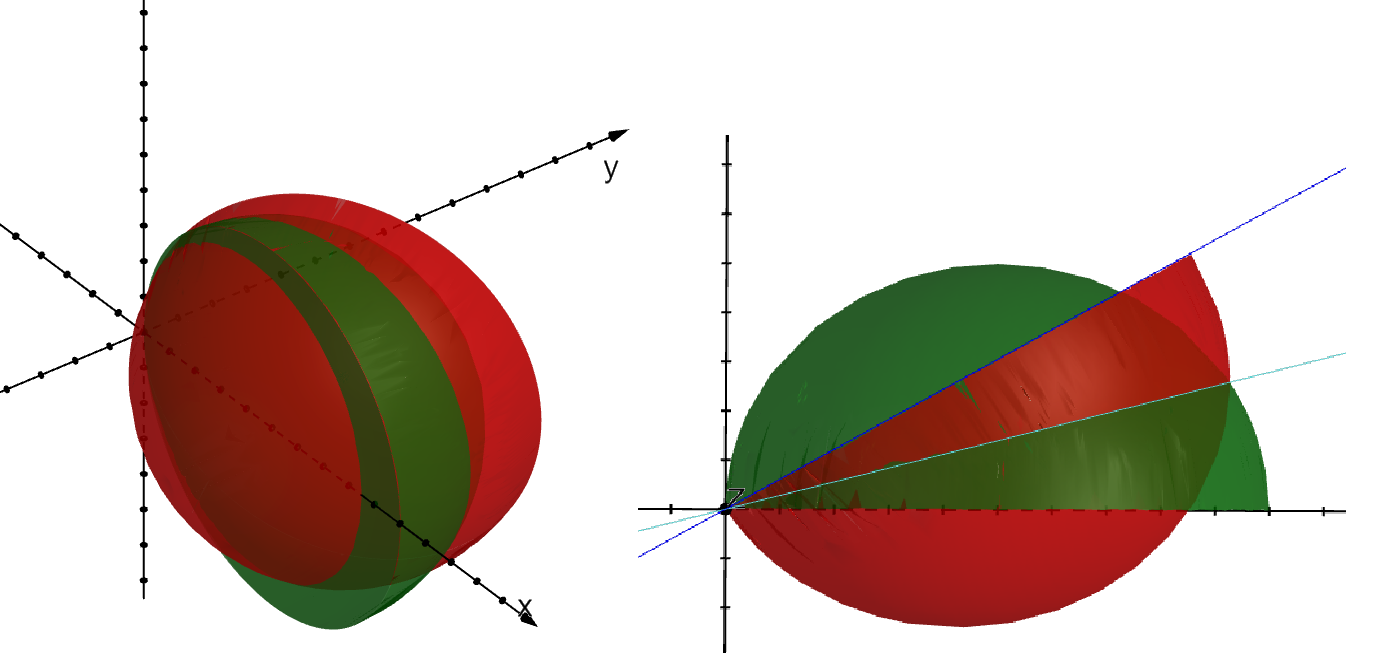
\includegraphics[width=0.7\linewidth]{../problems/Q_209/A_209_1.png}
\end{figure}

上図の緑半球が$A$、赤半球が$C$。

立体は平面$y=x\tan\theta$について対称なので、$y\ge x\tan\theta$の部分を考える。これは$A$のうち、平面$y=x\tan\theta$と$y=x\tan2\theta$によって囲まれる領域である。$0<t<\dfrac{\pi}{2}$に対し、$A$のうち$y\ge x\tan t$を満たす部分の体積を$f(t)$とおくと\footnote{編者註: 読みやすさのため関数記号を変更しました。}、求める体積は$V=f(\theta)-f(2\theta)$で表せる。

\begin{figure}[H]
 \centering
 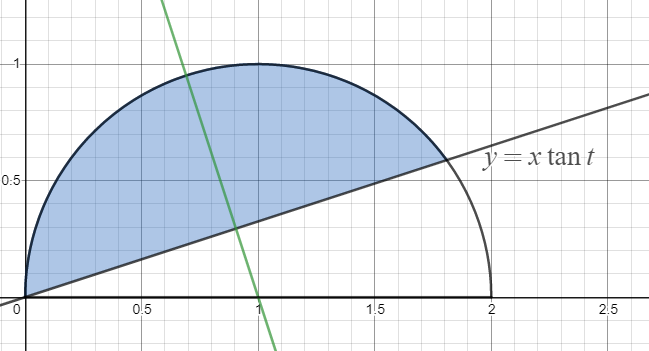
\includegraphics[width=0.6\linewidth]{../problems/Q_209/A_209_2.png}
\end{figure}

$f(t)$を計算する。$A$の平面$z=0$での断面 (右図) において、青色域を緑線を軸に回転させた領域の体積が$f(t)$となる。緑線を$w$軸とすれば、
\begin{align*}
 f(t)&=\int_{\sin t}^1\! \pi \left(\sqrt{1-w^2}\right)^2 \,dw = \pi\left(\frac{\sin^3 t}{3}-\sin t\right)+\frac{2}{3}\pi
\end{align*}
と求まる。これを用いて
\[ V=f(\theta)-f(2\theta)=\frac{\pi}{3}(\sin^3\theta-\sin^32\theta)-\pi(\sin \theta-\sin 2\theta) \]
となる。これを$\theta$で微分して、
\begin{align*}
 \frac{dV}{d\theta}&=\pi(\cos\theta\sin^2\theta-2\cos2\theta\sin^22\theta)-\pi(\cos\theta-2\cos2\theta) \\
 &= 2\pi\cos^32\theta-\pi\cos^3\theta \\
 &= \pi(\sqrt[3]{2}\cos2\theta-\cos\theta) \\
 &\qquad \times(\sqrt[3]{4}\cos^22\theta+\sqrt[3]{2}\cos2\theta\cos\theta+\cos^2\theta)
\end{align*}
を得る。$0<\theta<\dfrac{\pi}{4}$の範囲では最後の項は常に正だから、$\dfrac{dV}{d\theta}$の符号は$\sqrt[3]{2}\cos2\theta-\cos\theta$の正負によって決まる。$c=\cos\theta$についての2次関数$g=2\sqrt[3]{2}c^2-c-\sqrt[3]{2}$ (ただし$\frac{1}{\sqrt{2}}<c<1$) を考えれば、
\begin{align*}
 \frac{1}{\sqrt{2}}<c<\frac{\sqrt[3]{4}+\sqrt{32+2\sqrt[3]{2}}}{8}\,\text{のとき}\,&\frac{dV}{d\theta}<0 \\
 \frac{\sqrt[3]{4}+\sqrt{32+2\sqrt[3]{2}}}{8}<c<1\,\text{のとき}\,&\frac{dV}{d\theta}>0
\end{align*}
である。$\cos\alpha=\dfrac{\sqrt[3]{4}+\sqrt{32+2\sqrt[3]{2}}}{8}$となる$\alpha$ (ただし$0<\alpha<\dfrac{\pi}{4}$) をとる。$0<\theta<\dfrac{\pi}{4}$のとき、$\cos\theta$は単調減少することをふまえれば、$V$は$0<\theta<\alpha$で増加、$\alpha<\theta<\dfrac{\pi}{4}$で減少するから、$V$は$\theta=\alpha$のとき極大となる。

よって求める値は$\cos\alpha=\dfrac{\sqrt[3]{4}+\sqrt{32+2\sqrt[3]{2}}}{8}$